\chapter{Background}
\label{chap:background}

\section{The Quantum Threat and Public-Key Cryptography}

All widely deployed public-key cryptography relies on computational hardness assumptions. RSA depends on the difficulty of integer factorization; Diffie-Hellman and its elliptic-curve variants (including X25519, as used in WireGuard) depend on the discrete logarithm problem. No polynomial-time classical algorithm is known for any of these at cryptographic parameter sizes, and for decades that has been enough.

Shor's algorithm~\cite{shor1994algorithms} upends this. A fault-tolerant quantum computer with enough qubits can solve both integer factorization and discrete logarithm in polynomial time, an exponential speedup over the best classical approaches. Concretely, such a machine could derive an X25519 private key from the corresponding public key and reconstruct any session key derived from it. Gidney and Eker\aa~\cite{gidney2021factor} estimate that RSA-2048 could be factored with roughly 20 million noisy qubits in a matter of hours.

What makes this urgent is the harvest-now-decrypt-later (HNDL) attack model. An adversary who lacks a quantum computer today can still passively record encrypted traffic --- WireGuard handshakes, transport data, all of it --- and store it cheaply. Once a sufficiently powerful quantum computer is available, the adversary recovers the X25519 private keys from the stored public keys, reconstructs the ephemeral shared secrets, and decrypts everything. The uncomfortable implication is that traffic encrypted today with classical-only key exchange may already be compromised in a meaningful sense, even though the quantum computers needed to exploit it do not yet exist.

Symmetric cryptography, by contrast, is largely safe. Grover's algorithm provides only a quadratic speedup for brute-force search, effectively halving key lengths: AES-256 retains 128 bits of security against quantum adversaries, which is still more than adequate. ChaCha20-Poly1305, BLAKE2s, and the HMAC-based key derivation used by WireGuard are similarly unaffected. The migration problem is confined to the asymmetric key exchange layer.

NIST's response was a structured standardization effort that produced ML-KEM for key encapsulation, ML-DSA for signatures, and SLH-DSA for hash-based signatures. The accompanying transition timeline is concrete: classical key exchange (RSA, ECDH, ECDSA) is to be deprecated after 2030 and disallowed after 2035~\cite{nistir8547}. Organizations handling data that must remain confidential past 2035 face an even tighter deadline, since that data is already at risk from HNDL collection if protected only by classical key exchange today.

\section{WireGuard: Protocol Design and Architecture}

WireGuard~\cite{donenfeld2017wireguard} is a layer-3 VPN protocol built around a small set of modern cryptographic primitives and a deliberately minimal state machine. Donenfeld's design philosophy favours conservatism: a fixed cipher suite with no algorithm negotiation, a single round-trip handshake, and fewer than 4,000 lines of code in the reference implementation.

The core cryptographic design uses Trevor Perrin's Noise Protocol Framework~\cite{noise-protocol} for the handshake, specifically the IK pattern, combined with X25519 for Diffie-Hellman key exchange, HKDF~\cite{rfc5869} for key derivation, ChaCha20-Poly1305 for authenticated encryption of transport data, and BLAKE2s for hashing.

WireGuard's networking model is built around a concept called cryptokey routing: each peer is identified by a 32-byte Curve25519 public key, and the interface maintains a mapping from public keys to allowed IP address ranges. This means that IP-level authentication is cryptographically derived — any packet arriving on a WireGuard interface has a reliably authenticated source IP, provided the underlying session was established correctly.

The handshake produces a 1-RTT session. The initiator sends a first message that authenticates both the initiator's identity (via the static public key) and commits an ephemeral Curve25519 key. The responder verifies the initiator's identity, generates its own ephemeral key, and sends a response message. After the response is processed, both parties independently derive the same pair of symmetric session keys using HKDF. Transport data subsequently flows in UDP packets using ChaCha20-Poly1305 with a nonce counter.

\begin{figure}[!htbp]
    \centering
    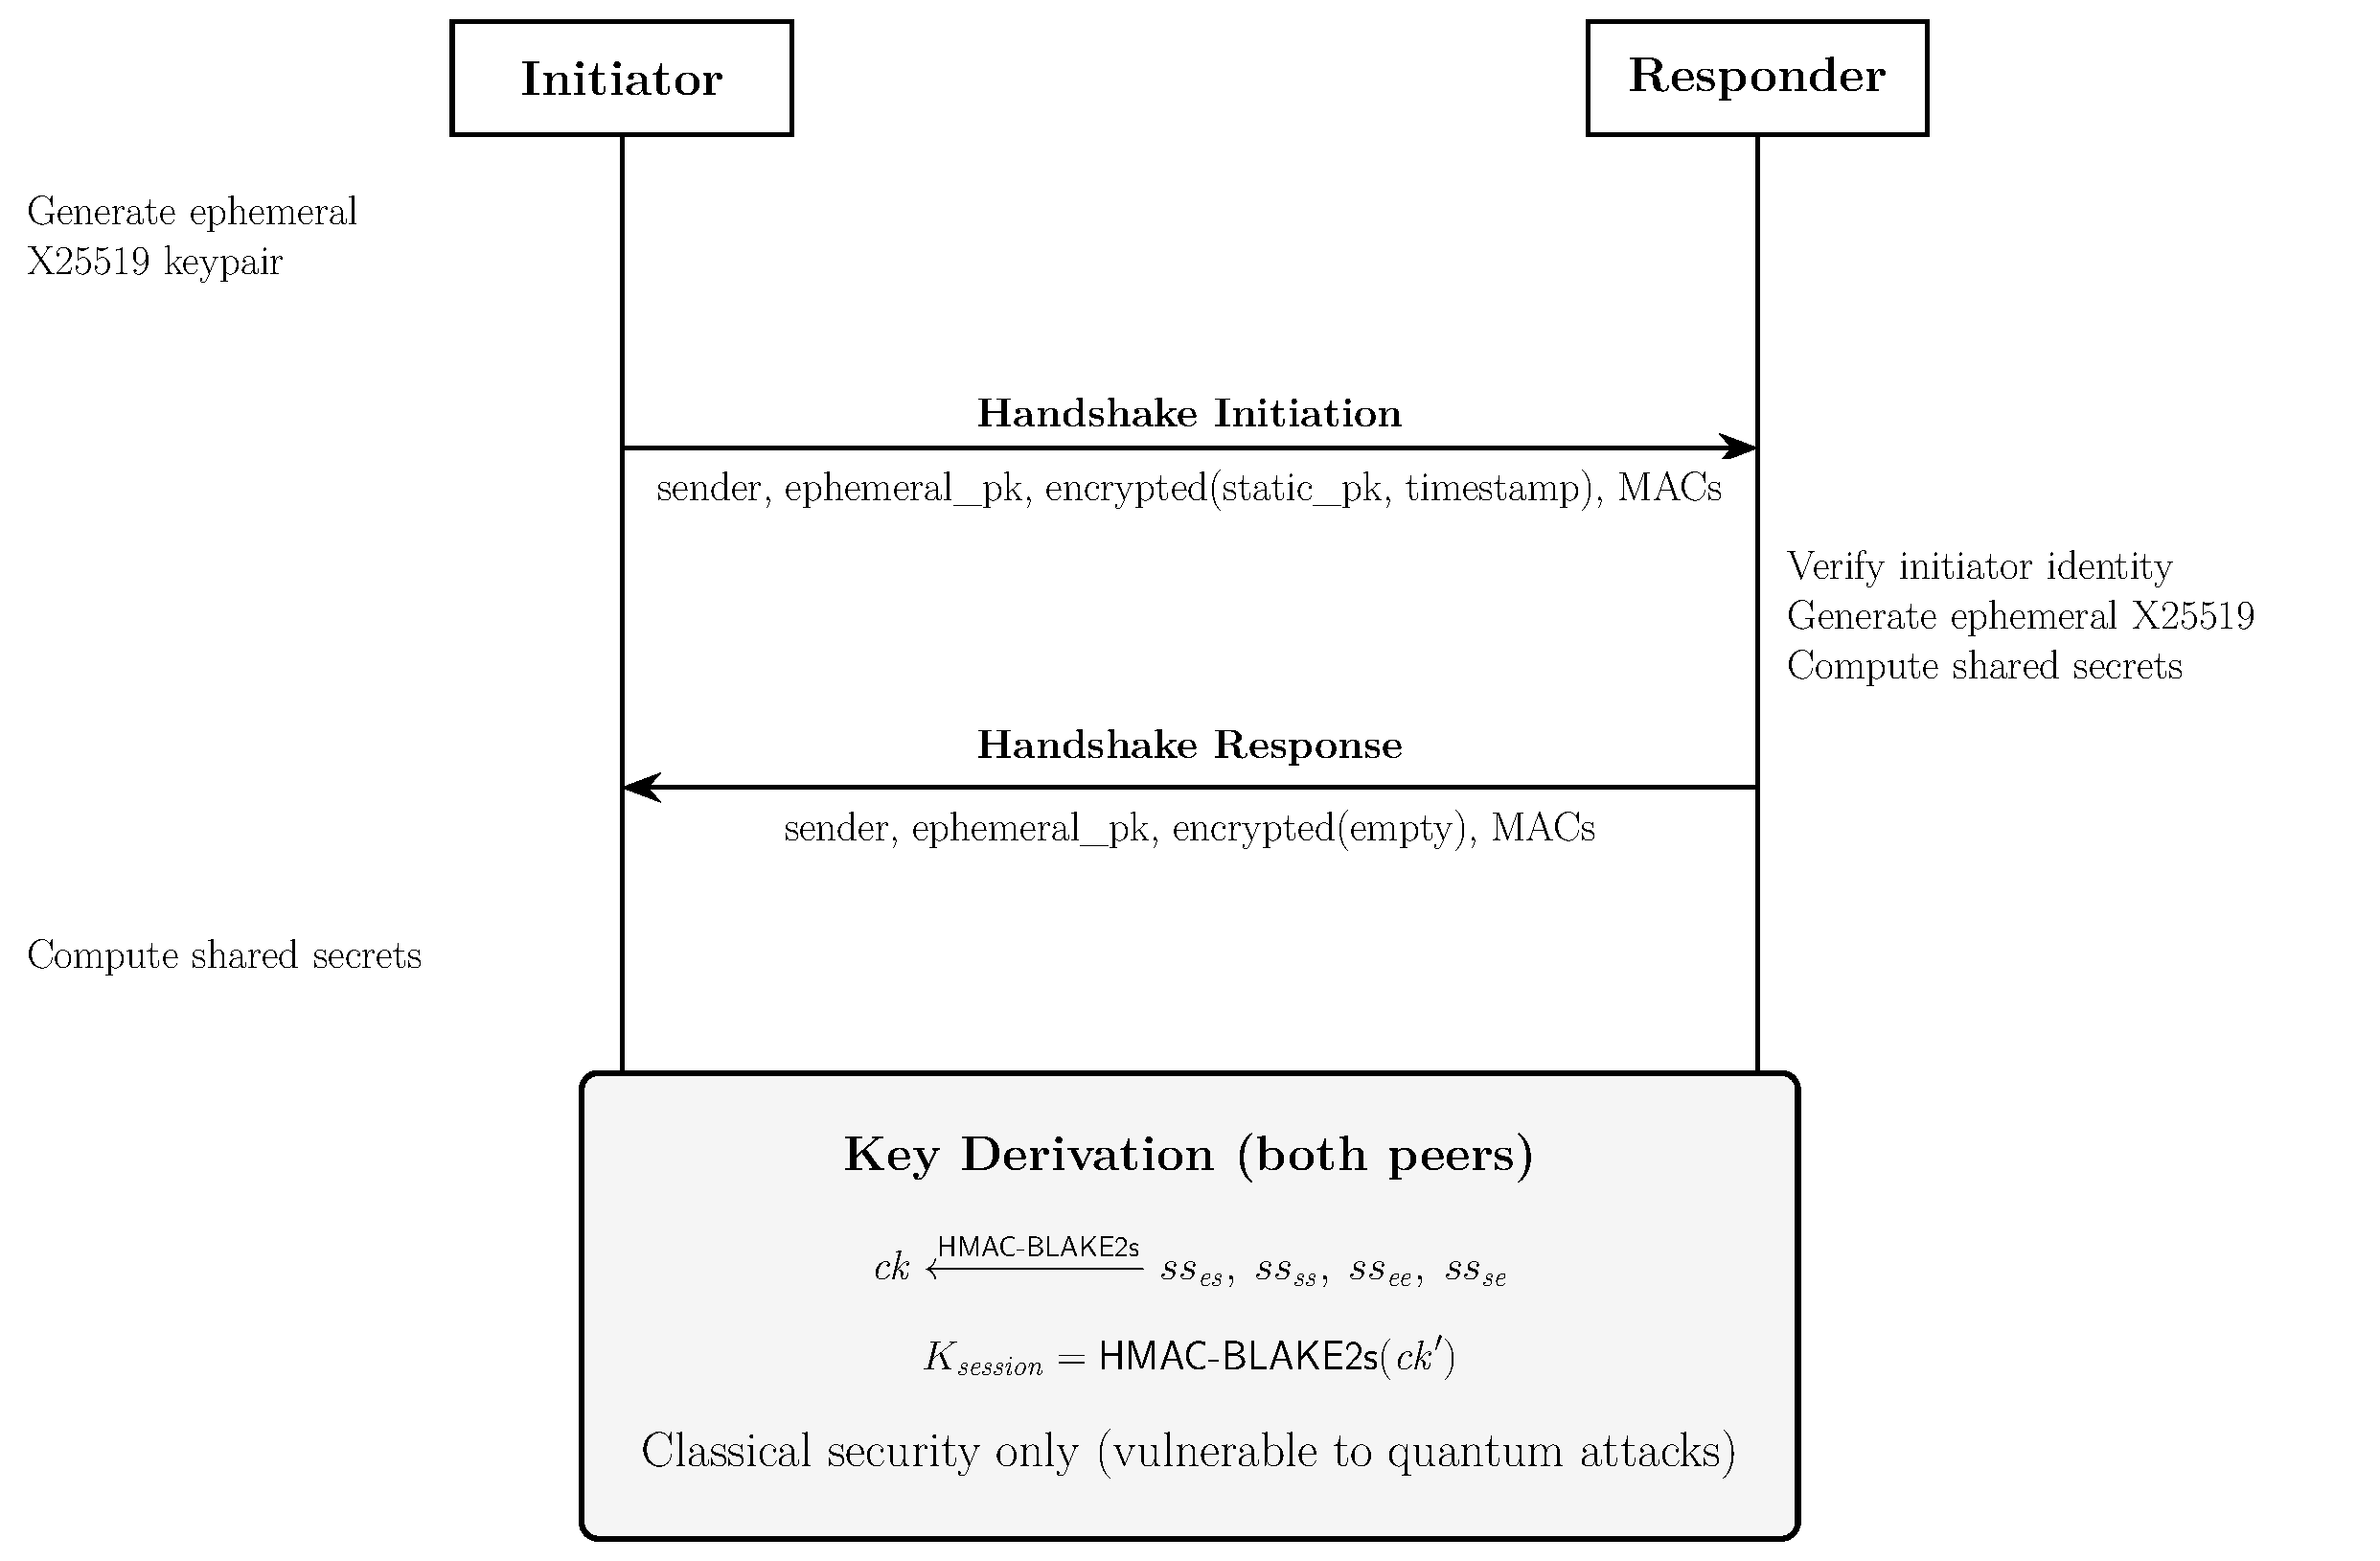
\includegraphics[width=\textwidth]{figures/fig_vanilla_handshake.pdf}
    \caption{Vanilla WireGuard Handshake (Noise IK pattern).}
    \label{fig:vanilla_handshake}
\end{figure}

WireGuard's timer state machine handles session lifecycle automatically: sessions rekey after 120 seconds or after 2\textsuperscript{60} transport messages, whichever comes first. All ephemeral keys and intermediate cryptographic material are zeroed from memory after use.

WireGuard also has unusually strong denial-of-service resistance. The responder never allocates state for unauthenticated packets, which makes it invisible to port scanners and limits the impact of resource-exhaustion attacks. When under load, a cookie mechanism lets the responder push work back to the initiator.

Performance-wise, WireGuard significantly outperforms legacy VPN protocols. Donenfeld's benchmarks show roughly 0.403ms ping times and the ability to saturate a gigabit Ethernet link, beating both OpenVPN and IPsec in AES-GCM and ChaCha20 modes.

\subsection{The PSK Slot}

WireGuard includes an optional pre-shared symmetric key (PSK) feature, added specifically to provide a measure of post-quantum protection. When configured, this 256-bit symmetric key is mixed into the HKDF key derivation chain during the handshake, adding a layer of symmetric-key cryptography on top of the X25519 exchange. The design intent is that even if a quantum computer eventually breaks X25519, an attacker who did not also obtain the PSK at the time of the session cannot decrypt the traffic.

The PSK mechanism was explicitly designed as a transitional measure for ``the extremely paranoid.'' Its limitations are structural: the PSK is a long-lived static value, not an ephemeral secret, so it does not provide forward secrecy for the quantum-resistant component. If the PSK itself is compromised — whether through theft, misconfiguration, or an insider — all sessions protected by it are retrospectively vulnerable. Distribution and rotation of PSKs also requires an out-of-band channel, shifting operational complexity to deployment teams.

\section{The Noise Protocol Framework}

Noise, designed by Trevor Perrin, is a framework for building authenticated key exchange protocols from a small set of cryptographic patterns. A Noise pattern specifies the sequence of messages exchanged between an initiator and a responder, along with the Diffie-Hellman operations performed at each step and the order in which public keys become known to each party.

WireGuard uses the IK pattern, named for how each party's static key is handled: \emph{I} for the initiator's static, which is transmitted \emph{immediately} during the handshake (encrypted, so passive eavesdroppers cannot see it), and \emph{K} for the responder's static, which is \emph{known} to the initiator beforehand. The pattern provides a one-round-trip mutually authenticated key exchange and identity hiding for the initiator's static against passive observers.

Noise protocols maintain two running state values: a chaining key (ck) and a handshake hash (h). Each DH operation, public key transmission, and encrypted payload is mixed into these values via HKDF and BLAKE2s, building a transcript hash that cryptographically binds all handshake messages together. The session keys at the end of the handshake are derived from the final value of ck.

The main difficulty in migrating Noise to post-quantum cryptography is that its design is deeply tied to the algebraic properties of Diffie-Hellman. DH provides non-interactive key exchange: the initiator can compute $g^{ab}$ from the responder's public key $g^b$ and its own private key $a$, and vice versa, without any interaction. KEMs work differently: one party generates a ciphertext that encapsulates a secret to a specific public key, and only the holder of the corresponding private key can decapsulate it. This asymmetry means the handshake flow needs to be reworked when KEMs are introduced.

\begin{figure}[!htbp]
    \centering
    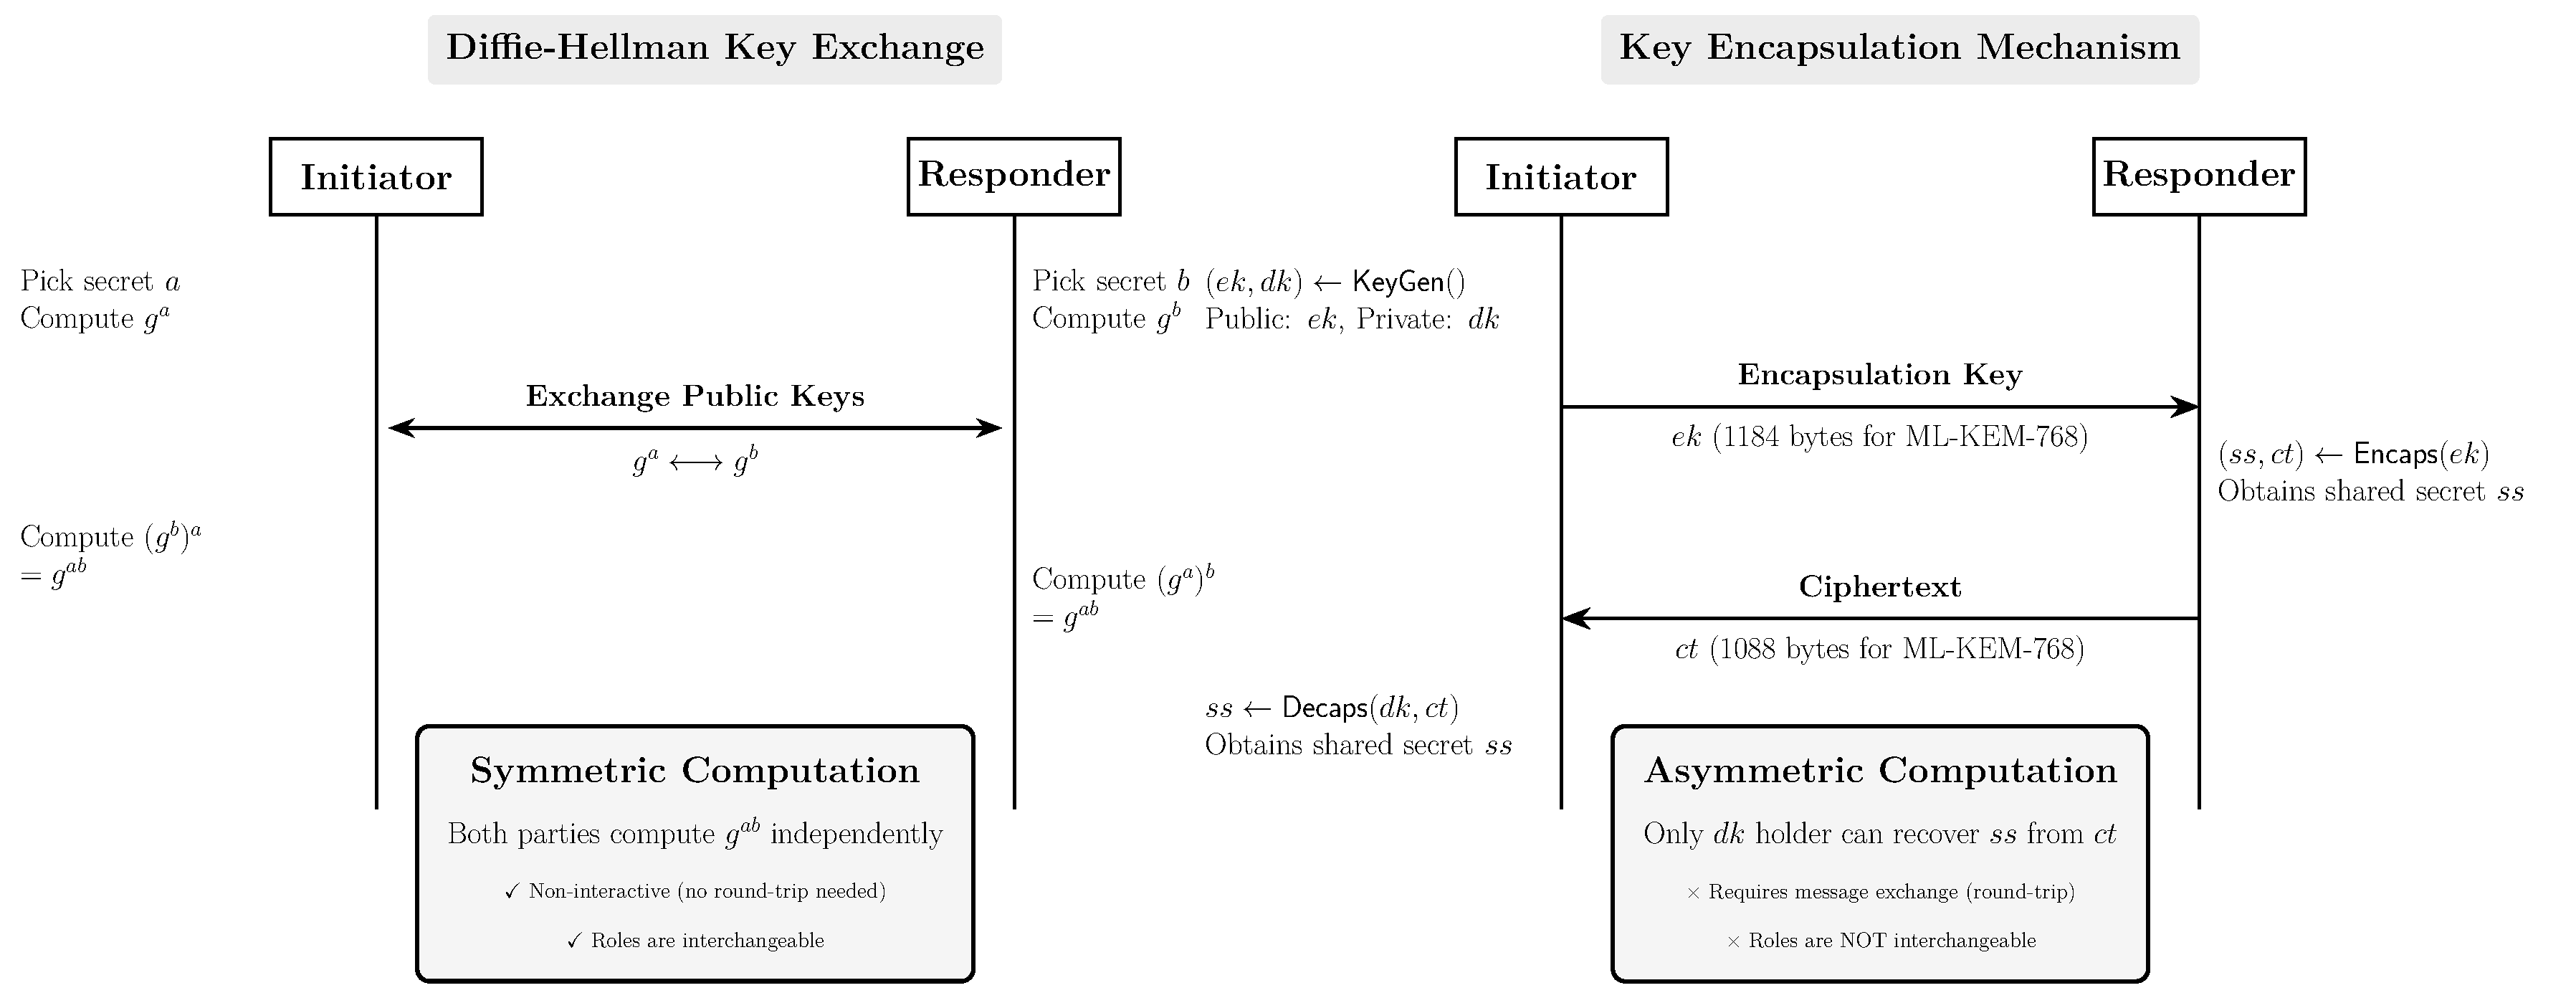
\includegraphics[width=\textwidth]{figures/fig_kem_vs_dh.pdf}
    \caption{Comparison of Diffie-Hellman key exchange and Key Encapsulation Mechanisms, illustrating the asymmetry challenge for Noise protocol migration. The KEM side shows the canonical direction, where the recipient of the shared secret publishes the encapsulation key; the hybrid construction in Chapter~\ref{chap:design} runs this the other way around, with the initiator generating an ephemeral $(\mathit{ek}, \mathit{dk})$ and sending $\mathit{ek}$ in the first message to mirror the X25519 ephemeral flow.}
    \label{fig:kem_vs_dh}
\end{figure}

\section{ML-KEM (FIPS 203)}

ML-KEM was standardized as FIPS 203 in August 2024~\cite{fips203}. It is a key encapsulation mechanism derived from CRYSTALS-Kyber~\cite{bos2018crystals}, whose 2018 EuroS\&P paper was authored by Bos, Ducas, Kiltz, Lepoint, Lyubashevsky, Schanck, Schwabe, Seiler, and Stehl\'{e}; Avanzi, Ding, and others joined the broader NIST Kyber submission team.

A KEM exposes three operations: KeyGen produces an encapsulation key and a decapsulation key; Encaps takes an encapsulation key and returns a ciphertext plus a shared secret; Decaps takes the decapsulation key and the ciphertext and recovers the same shared secret. Correctness is guaranteed as long as randomness generation is sound.

The security of ML-KEM rests on the Module Learning With Errors (MLWE) problem, introduced by Regev in 2005 and generalized to module lattices by Langlois and Stehlé~\cite{langlois2015worst}. The MLWE problem asks: given a matrix A, vectors $b = As + e$ for small error $e$ and secret $s$, distinguish $(A, b)$ from uniform random. No efficient quantum algorithm is known for this problem; the best attacks remain classical lattice reduction algorithms whose complexity scales superpolynomially with the security parameter.

ML-KEM is constructed in two steps. First, a public-key encryption scheme K-PKE is built from the MLWE problem. K-PKE is IND-CPA secure --- that is, secure against chosen-plaintext attacks --- but not IND-CCA2 secure. The IND-CCA2 security required for use in key exchange is obtained by applying a variant of the Fujisaki-Okamoto transform, which converts the PKE scheme into a KEM with the stronger security guarantee. The construction has been the target of several formal verification efforts, with machine-checked proofs of the FO transform and of Kyber-like schemes carried out in EasyCrypt and other proof assistants.

FIPS 203 specifies three parameter sets: ML-KEM-512 (NIST security category 1, equivalent to AES-128), ML-KEM-768 (category 3, equivalent to AES-192), and ML-KEM-1024 (category 5, equivalent to AES-256). The key and ciphertext sizes are as follows: ML-KEM-512 has a 800-byte encapsulation key and 768-byte ciphertext; ML-KEM-768 has a 1,184-byte encapsulation key and 1,088-byte ciphertext; ML-KEM-1024 has a 1,568-byte encapsulation key and 1,568-byte ciphertext. All three produce a 32-byte shared secret. NIST recommends ML-KEM-768 as the default parameter set, providing a large security margin at reasonable performance cost.

On the implementation side, ML-KEM benefits from the Number-Theoretic Transform (NTT), which makes polynomial multiplication efficient and gives ML-KEM a raw speed advantage over elliptic-curve operations. Benchmarks on Intel Xeon hardware show Kyber-768 key generation, encapsulation, and decapsulation each running roughly 2--3$\times$ faster than the corresponding X25519 operations in CPU cycles. In practice, though, this speed advantage is offset by the much larger key and ciphertext sizes, which tend to dominate handshake time whenever the network is the bottleneck.

\section{Hybrid Key Exchange and the Concatenate-then-KDF Pattern}

Hybrid key exchange combines two or more key agreement algorithms so that the resulting key is secure as long as at least one component holds. The motivation is straightforward: ML-KEM, though now standardized, is far newer than X25519 and has seen less cryptanalytic scrutiny. Running both in parallel means a breakthrough against either one alone does not compromise security.

The standard construction is the concatenate-then-KDF pattern, formalized in NIST SP 800-56C Rev. 2~\cite{nist-sp800-56c}. SP 800-56C explicitly permits hybrid shared secrets of the form $Z' = Z \| T$, a concatenation of a ``standard'' shared secret $Z$ (e.g., from X25519) and an auxiliary shared secret $T$ (e.g., from ML-KEM), fed into a single key derivation function. Giacon, Heuer, and Poettering~\cite{giacon2018combiners} prove that the resulting KEM is IND-CPA-secure as long as either component is IND-CPA-secure, with the bound remaining tight even when one component is completely broken.

This is the same pattern used by Cloudflare and Google in TLS 1.3 and by the IETF hybrid TLS design draft, which specifies X25519+ML-KEM hybrid groups for TLS key exchange~\cite{ietf-tls-hybrid-design}.
